\section{Resultados}
% Eu sei precisa colocar a imagem ajustar a imagem, mas calma, não sufoca o artista

\subsection{Quantificação e pureza do DNA}
A quantificação do DNA genômico foi realizada por espectrofotometria utilizando equipamento NanoDrop, 
com análise das razões de absorbância A\textsubscript{260}/A\textsubscript{280} e A\textsubscript{260}/A\textsubscript{230}. 
A amostra analisada apresentou concentração de 140{,}1~ng/µL, com razão A\textsubscript{260}/A\textsubscript{280} de 2{,}07 e 
A\textsubscript{260}/A\textsubscript{230} de 2{,}31. Esses valores indicam alta pureza, com ausência significativa de contaminantes 
como proteínas (razão esperada entre 1{,}8 e 2{,}0) ou compostos orgânicos/sais (razão A\textsubscript{260}/A\textsubscript{230} 
ideal > 1{,}8)\cite{Alguém}. A qualidade do DNA obtido foi considerada adequada para as reações de PCR subsequentes.

\subsection{Análise por PCR convencional}
A identificação molecular da amostra-problema foi conduzida por meio de três reações de PCR convencionais, designadas como PCR-A, PCR-B 
e PCR-C, cada uma com especificidade crescente em relação ao táxon de interesse. Os produtos amplificados foram analisados por eletroforese 
em gel de agarose a 1{,}5\%, conforme apresentado nas Figuras~\ref{pcrA} e~\ref{pcrBC}.

\begin{wrapfigure}{L}{.45\textwidth}
 \centering
 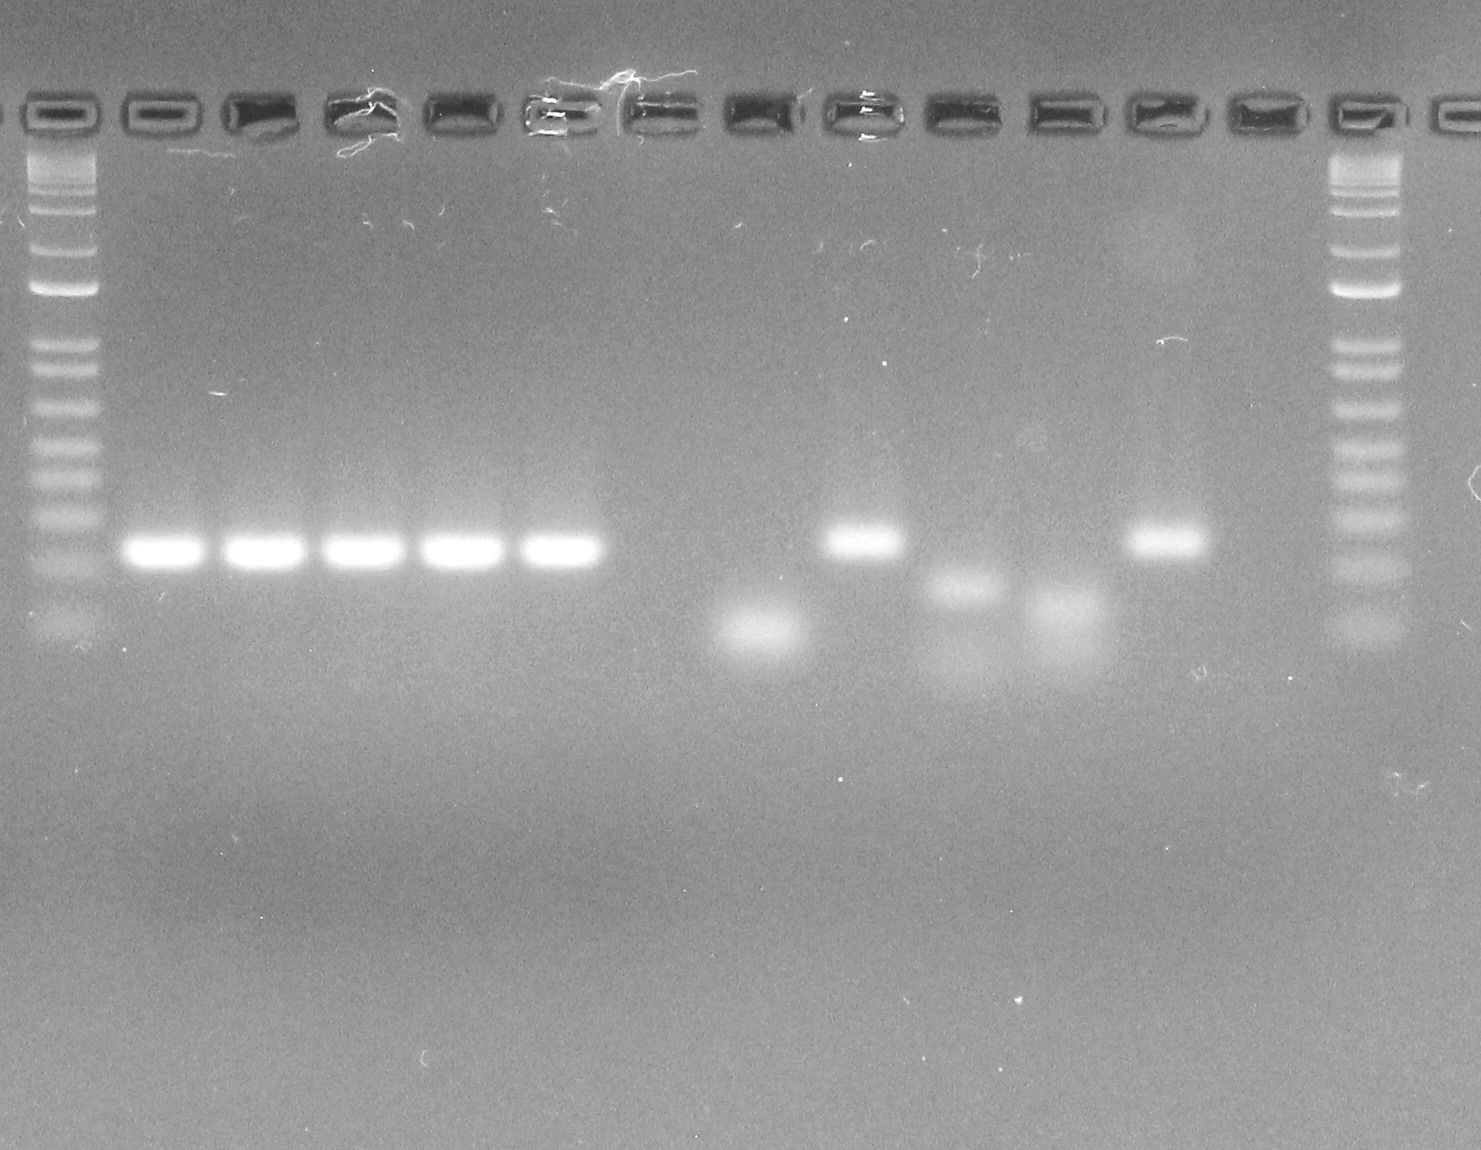
\includegraphics[width=.4\textwidth]{fig/pcrA_rflp_g8}
 \caption{Eletroforese dos produtos da PCR-A (gênero específico). As extremidades do gel contém escadas de peso molecular (ladders). 
 Os primeiros cinco poços da esquerda correspondem às amostras de DNA testadas quanto à presença do gênero \textit{Leishmania}, 
 seguidos por um controle negativo (água). Os poços subsequentes contêm, respectivamente: (1) \textit{L. (L.) infantum}, 
 (2) \textit{L. (L.) amazonensis}, (3) \textit{L. (V.) braziliensis}, (4) \textit{L. (V.) shawi}, (5) amostra-problema (W) e (6) controle negativo.}
 \label{pcrA}
 \end{wrapfigure}

A Figura~\ref{pcrA_rflp_g8} apresenta os resultados da eletroforese em gel de agarose referente à PCR-A, que tem como alvo uma região conservada do DNA genômico do gênero
 \textit{Leishmania}. Esta reação teve como objetivo inicial confirmar se a amostra-problema pertencia ao gênero, além de compará-la com amostras de referência previamente 
 caracterizadas. Observa-se que tanto a amostra-problema (poço 5) quanto a amostra-controle de \textit{L. (L.) amazonensis} (poço 2) apresentaram bandas com o mesmo tamanho 
 molecular e intensidade semelhante. Esse padrão sugere fortemente que a amostra W pertence à mesma espécie ou, no mínimo, ao mesmo subgênero da amostra-controle. Por outro 
 lado, as demais amostras  exibiram perfis distintos, e os controles negativos (poços 6 e 12) não apresentaram amplificação, confirmando a ausência de contaminações cruzadas.
Esses dados sustentam a hipótese de que a amostra-problema pertence ao gênero \textit{Leishmania}, com forte indício de pertencimento à espécie \textit{L. (L.) amazonensis}, 
conforme indicado pela coincidência do perfil eletroforético com a amostra-controle correspondente.

\begin{wrapfigure}{R}{.45\textwidth}
 \centering
 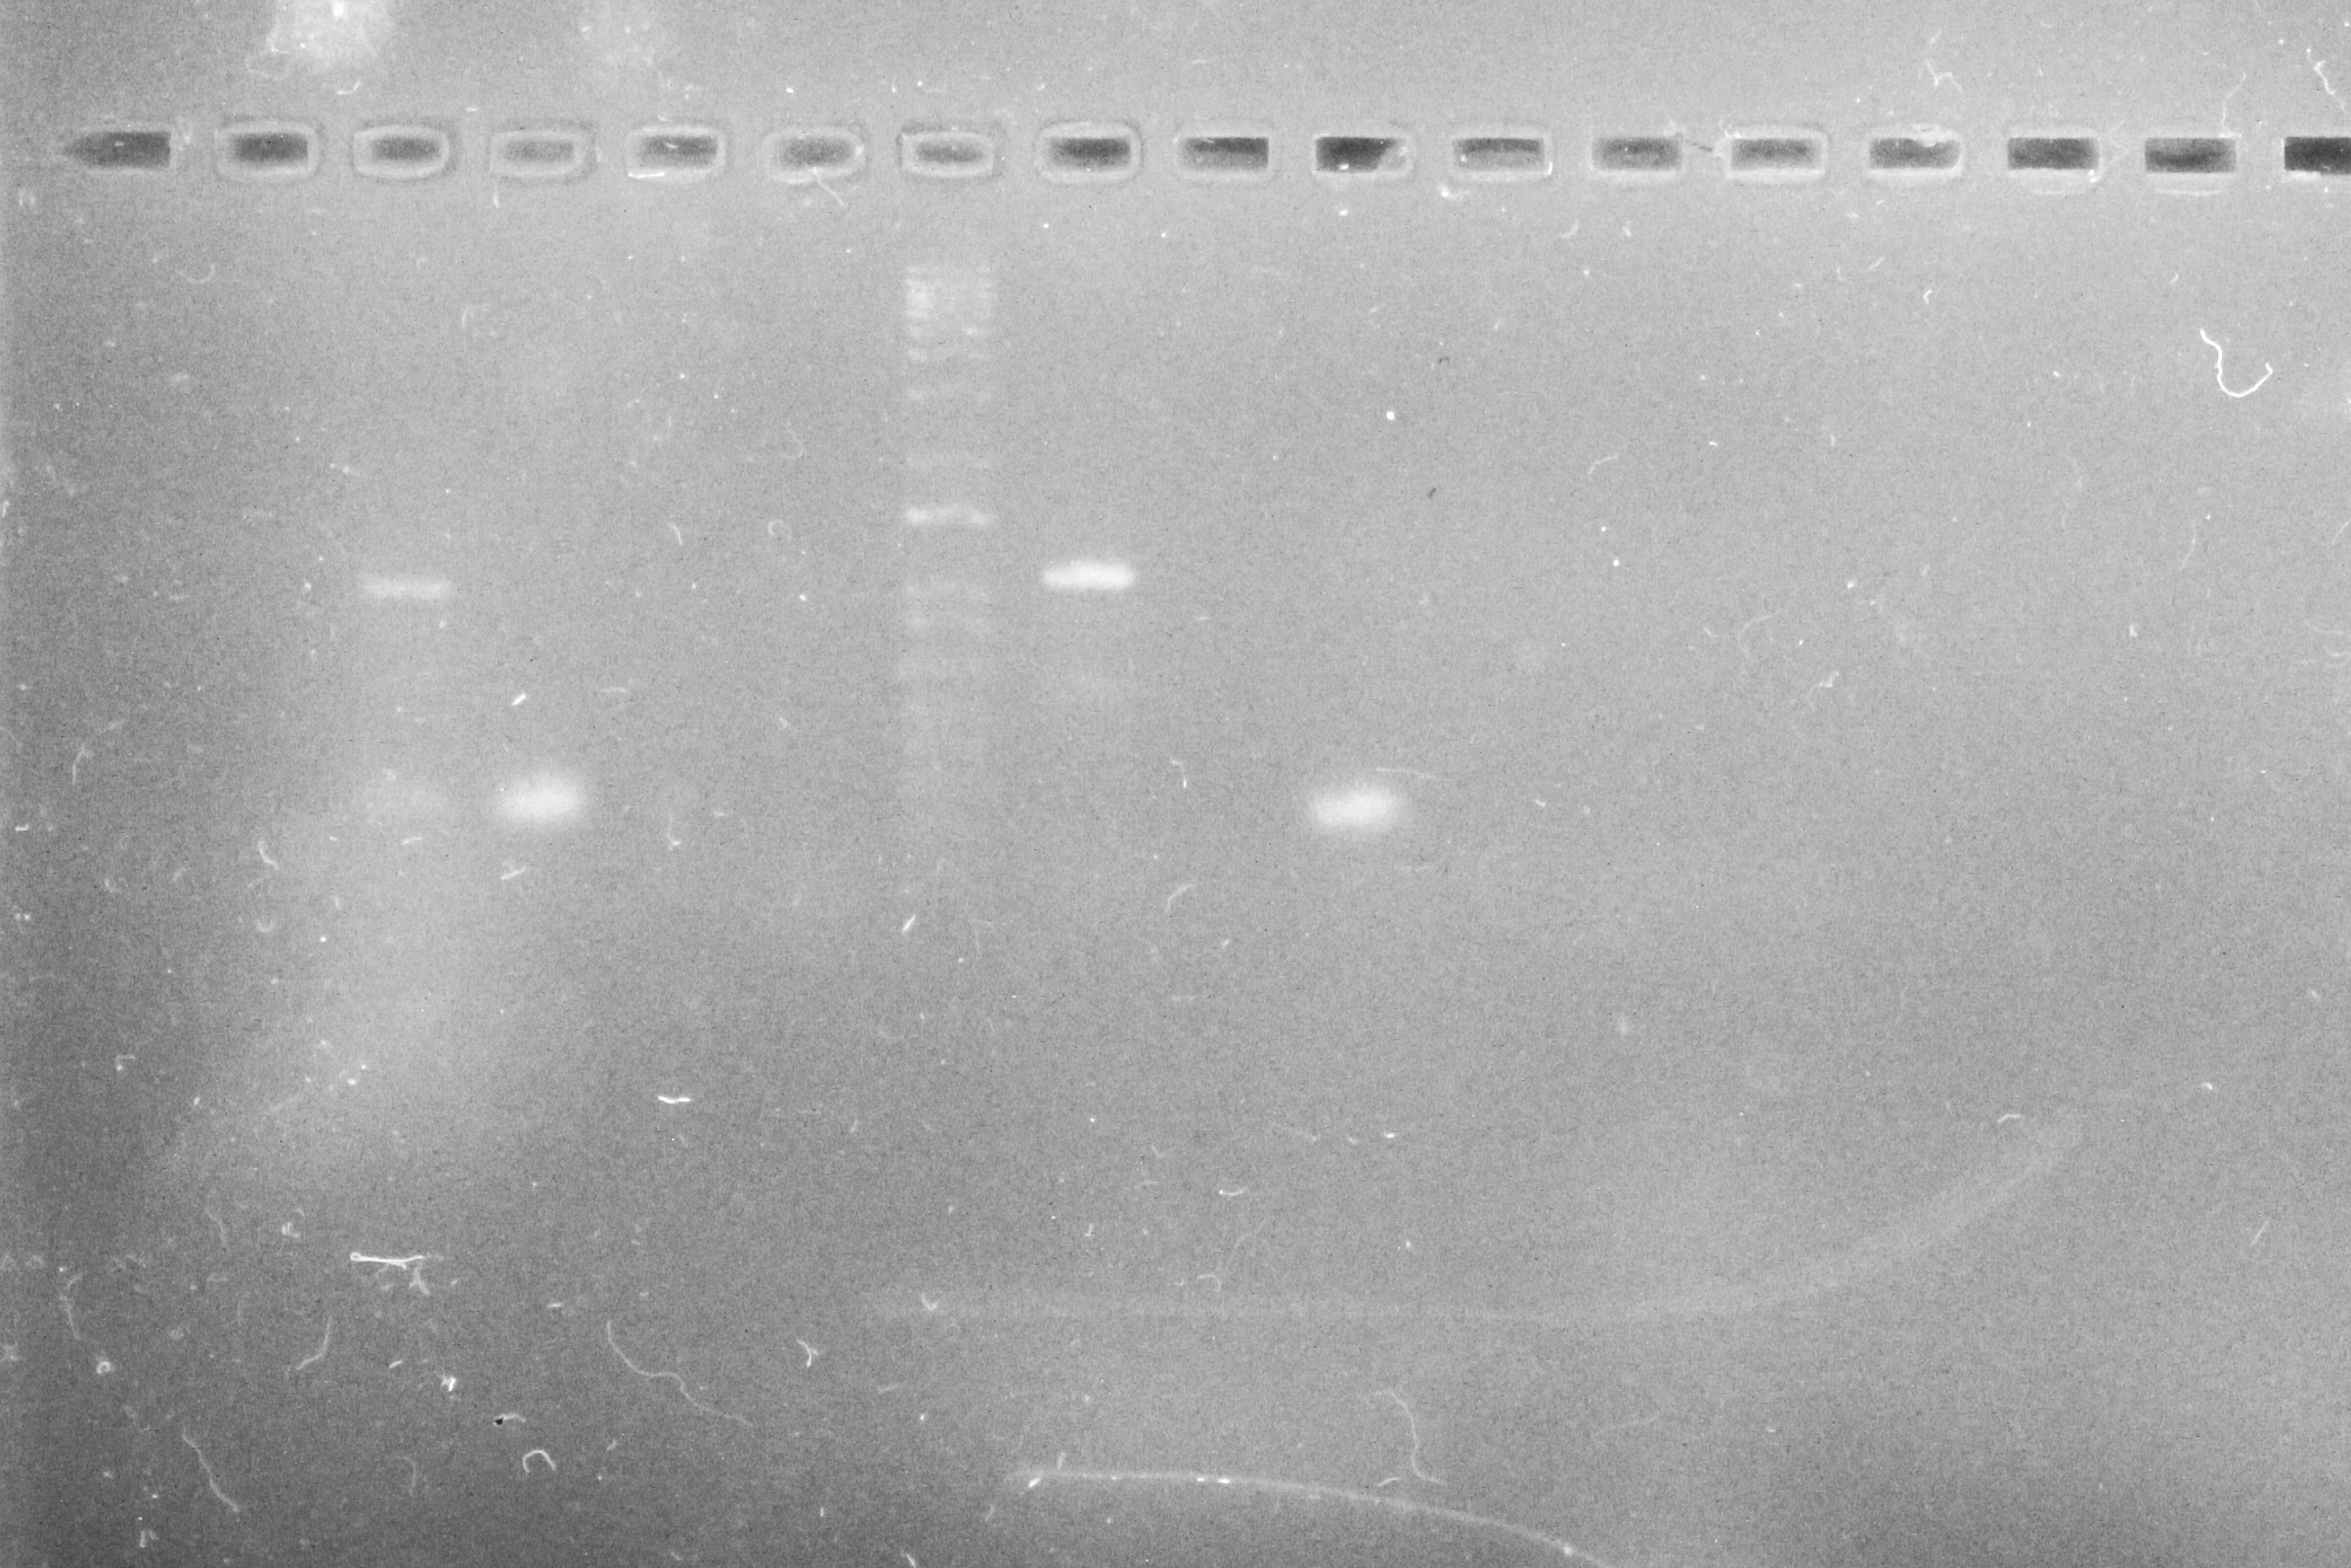
\includegraphics[width=.4\textwidth]{fig/pcrBeC_g8.jpg}
 \caption{Eletroforese dos produtos da PCR-B (subgênero \textit{Viannia}) e PCR-C (espécies não-\textit{braziliensis} do subgênero \textit{Viannia}). 
 A primeira série de seis poços à esquerda refere-se à PCR-B; em seguida há um poço com escada de peso molecular (ladder), seguido por seis poços referentes 
 à PCR-C. A ordem das amostras em ambas as reações é: (1) \textit{L. (L.) infantum}, (2) \textit{L. (L.) amazonensis}, (3) \textit{L. (V.) braziliensis}, 
 (4) \textit{L. (V.) shawi}, (5) amostra-problema (W) e (6) controle negativo.}
 \label{pcrBC}
 \end{wrapfigure}

As reações subsequentes, PCR-B e PCR-C representadas na Figura~\ref{pcrBeC_g8}, foram desenhadas com primers específicos para o subgênero \textit{Leishmania (Viannia)} e para espécies não-\textit{brasiliensis} dentro 
deste subgênero, respectivamente. Em ambas as reações, a amostra W não apresentou bandas detectáveis, ao contrário dos controles positivos específicos para \textit{L. (Viannia) 
braziliensis} e outras espécies do subgênero. A ausência de amplificação nas PCRs B e C reforça que a amostra W não pertence ao subgênero \textit{Viannia}, corroborando a classificação 
como \textit{Leishmania (Leishmania) amazonensis} já inferida pela PCR-A.

Na PCR-B, específica para o subgênero não-\textit{Leishmania (Viannia)}, foi observada uma banda nítida no poço 4, correspondente à amostra \textit{L. (V.) shawi}, como esperado. 
No entanto, uma banda mais tênue e não prevista foi detectada no poço 3, referente a \textit{L. (V.) braziliensis}, o que pode indicar uma amplificação inespecífica possivelmente causado
por erro no \textit{melting temperature(Tm)} visto que toda a placa ficou sob uma mesma temperatura e cada primer possuia um Tm específico. As demais amostras, incluindo a amostra-problema 
(poço 5), não apresentaram bandas visíveis, sugerindo ausência de amplificação com os primers utilizados nesta reação.

<<<<<<< HEAD
Já na PCR-C, voltada à detecção de espécies \textit{braziliensis} dentro do subgênero \textit{Viannia}, foi identificada uma banda clara no poço 3 (L. (V.) \textit{braziliensis}), 
como previsto. No entanto, uma amplificação não esperada foi observada no poço 1, correspondente a \textit{L. (L.) infantum}, o que novamente sugere a possibilidade de amplificação inespecífica.
Ambos os controles negativos dos PCR-B e PCR-C (amostra 6 em ambos) não foram amplificados, o que indica que não houve contaminação dos experimentos.
=======
Já na PCR-C, voltada à detecção de espécies \textit{braziliensis} dentro do subgênero \textit{Viannia}, foi identificada uma banda clara no poço 3 (L. (V.) braziliensis}), 
como previsto. No entanto, uma amplificação não esperada foi observada no poço 1, correspondente a \textit{L. (L.) infantum}, o que sugere a possibilidade de reação cruzada ou mínima 
contaminação da amostra.

\subsection{PCR em tempo real acomplado a High Resolution Melting Analysis}

A análise de HRM permite distinguir variantes de DNA com base em suas curvas de
dissociação térmica. As curvas de melting foram obtidas com o software High
Resolution Melt v.3.0.1 (Life Technologies), após a amplificação por PCR em
tempo real.

\begin{wrapfigure}{R}{.45\textwidth}
        \centering
        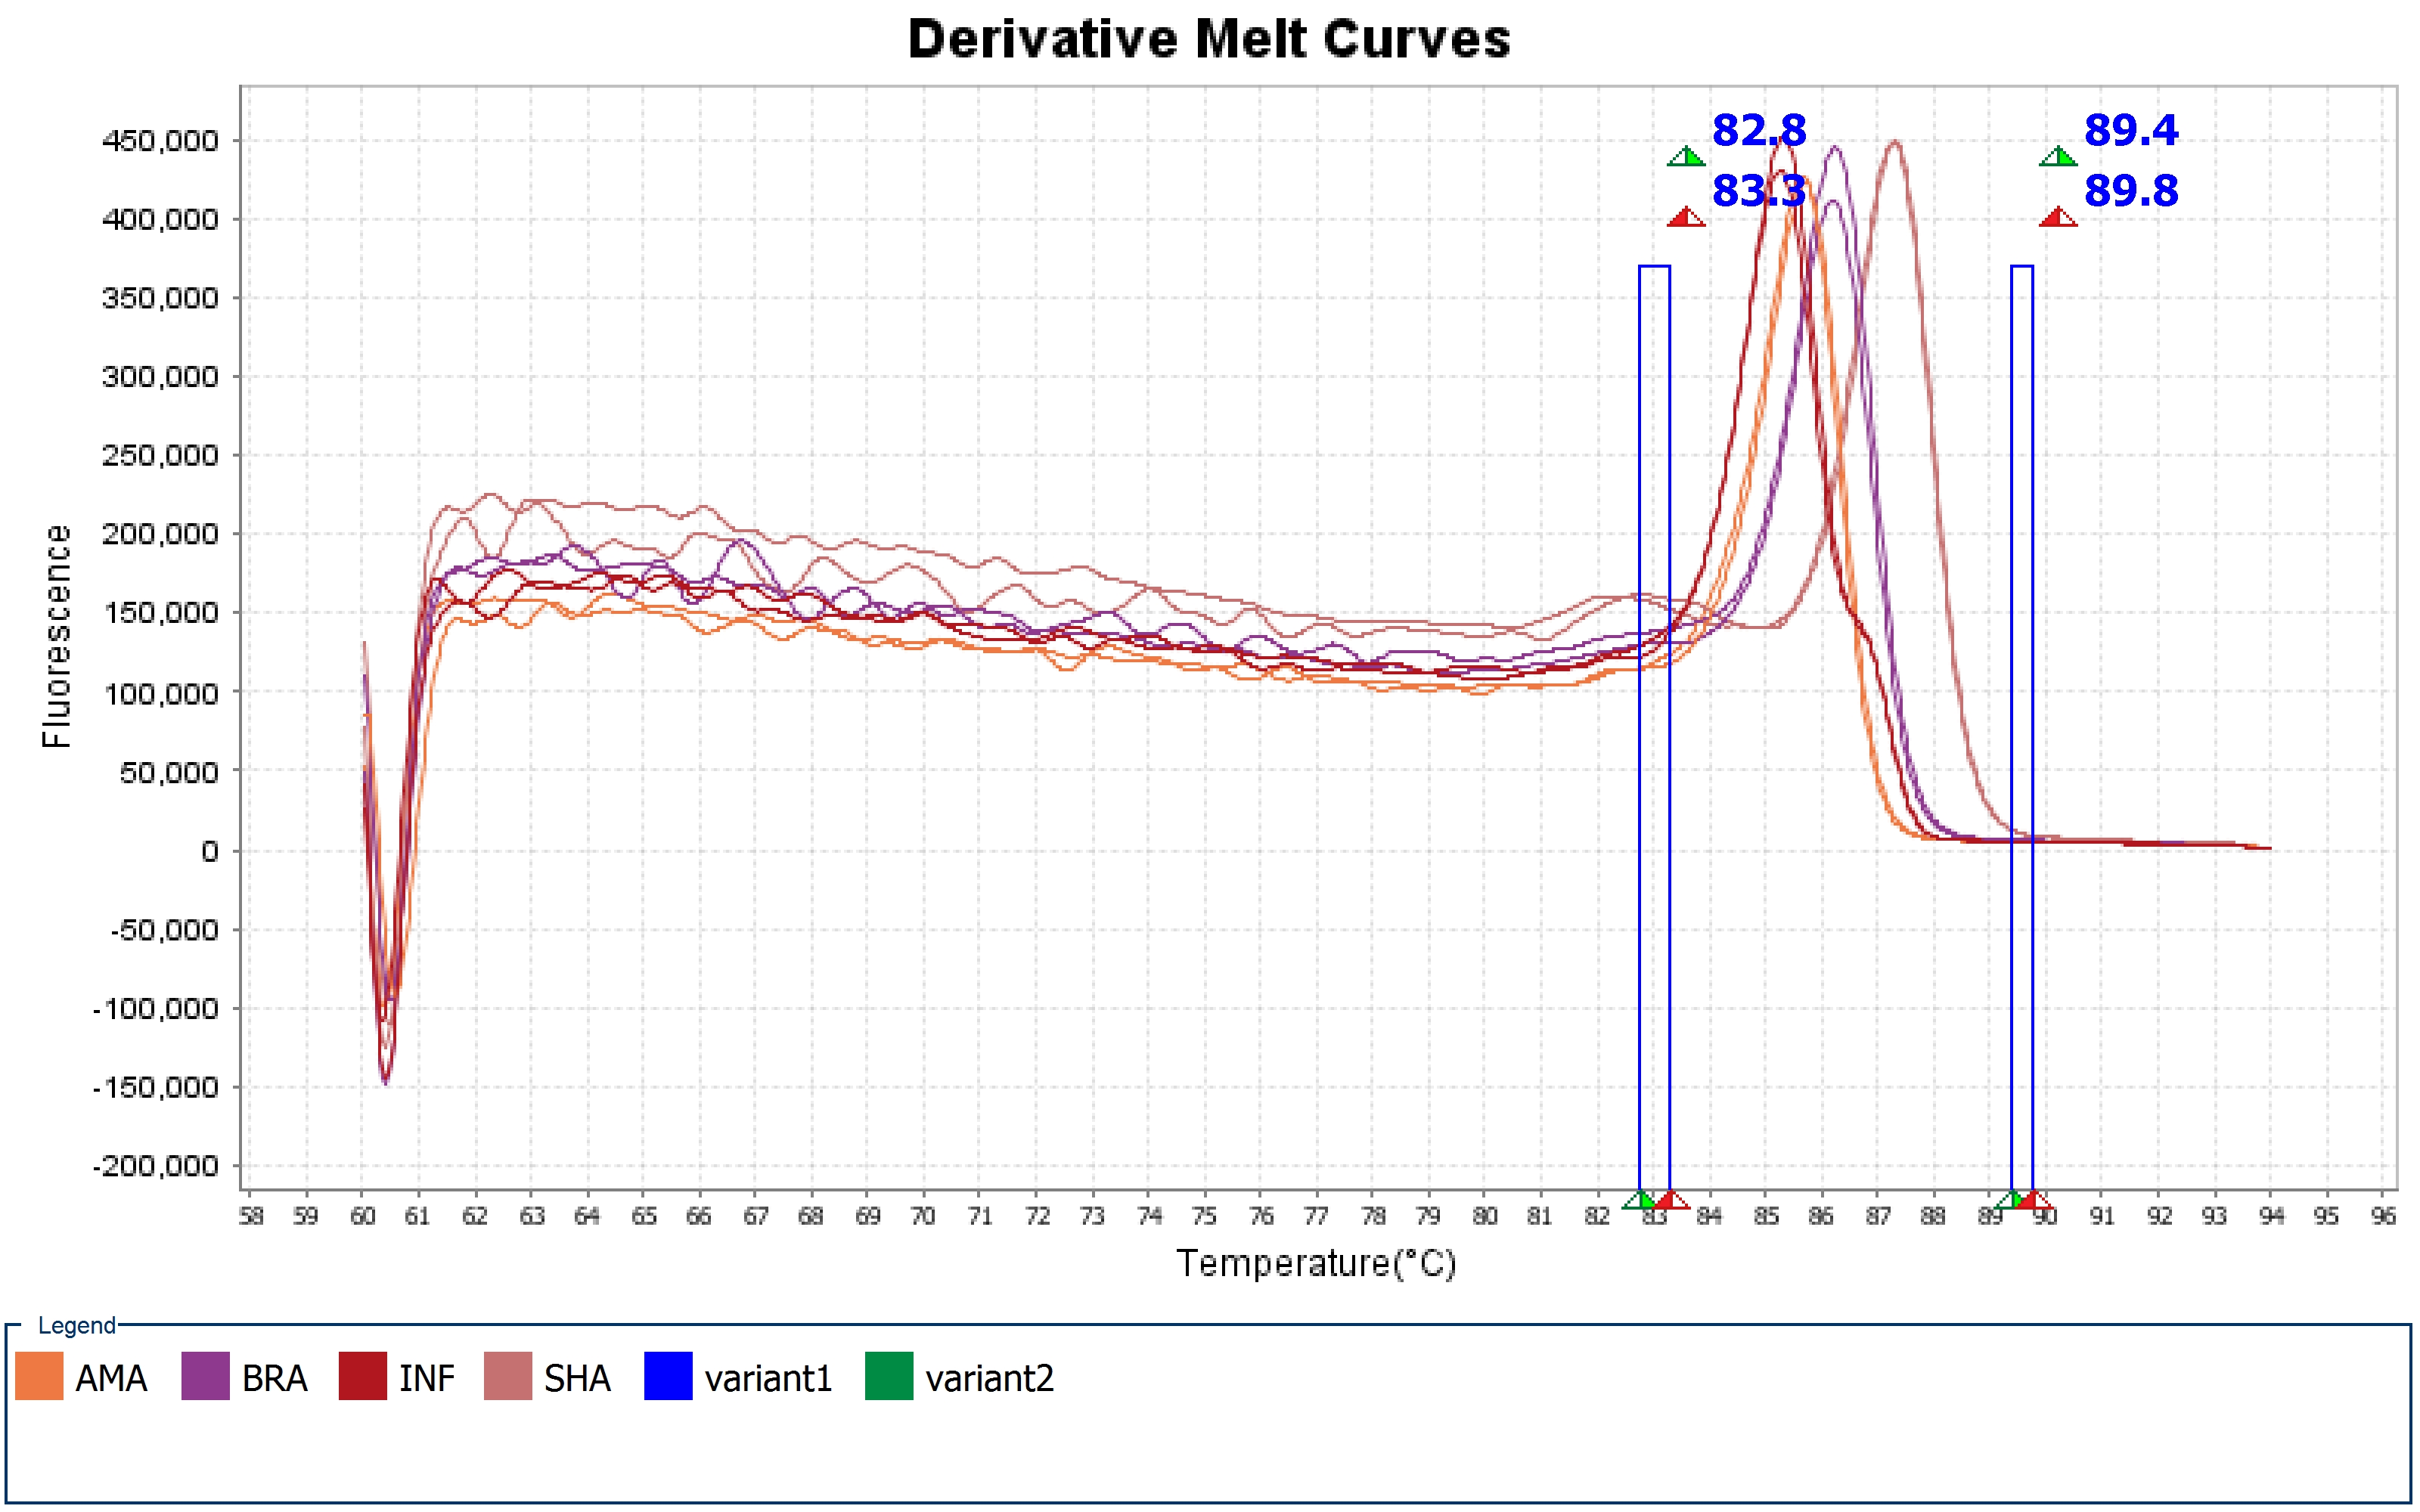
\includegraphics[width=.4\textwidth]{fig/Derivative Melt Curves.jpg}
        \caption{foto 1}
        \label{dmeltc}
        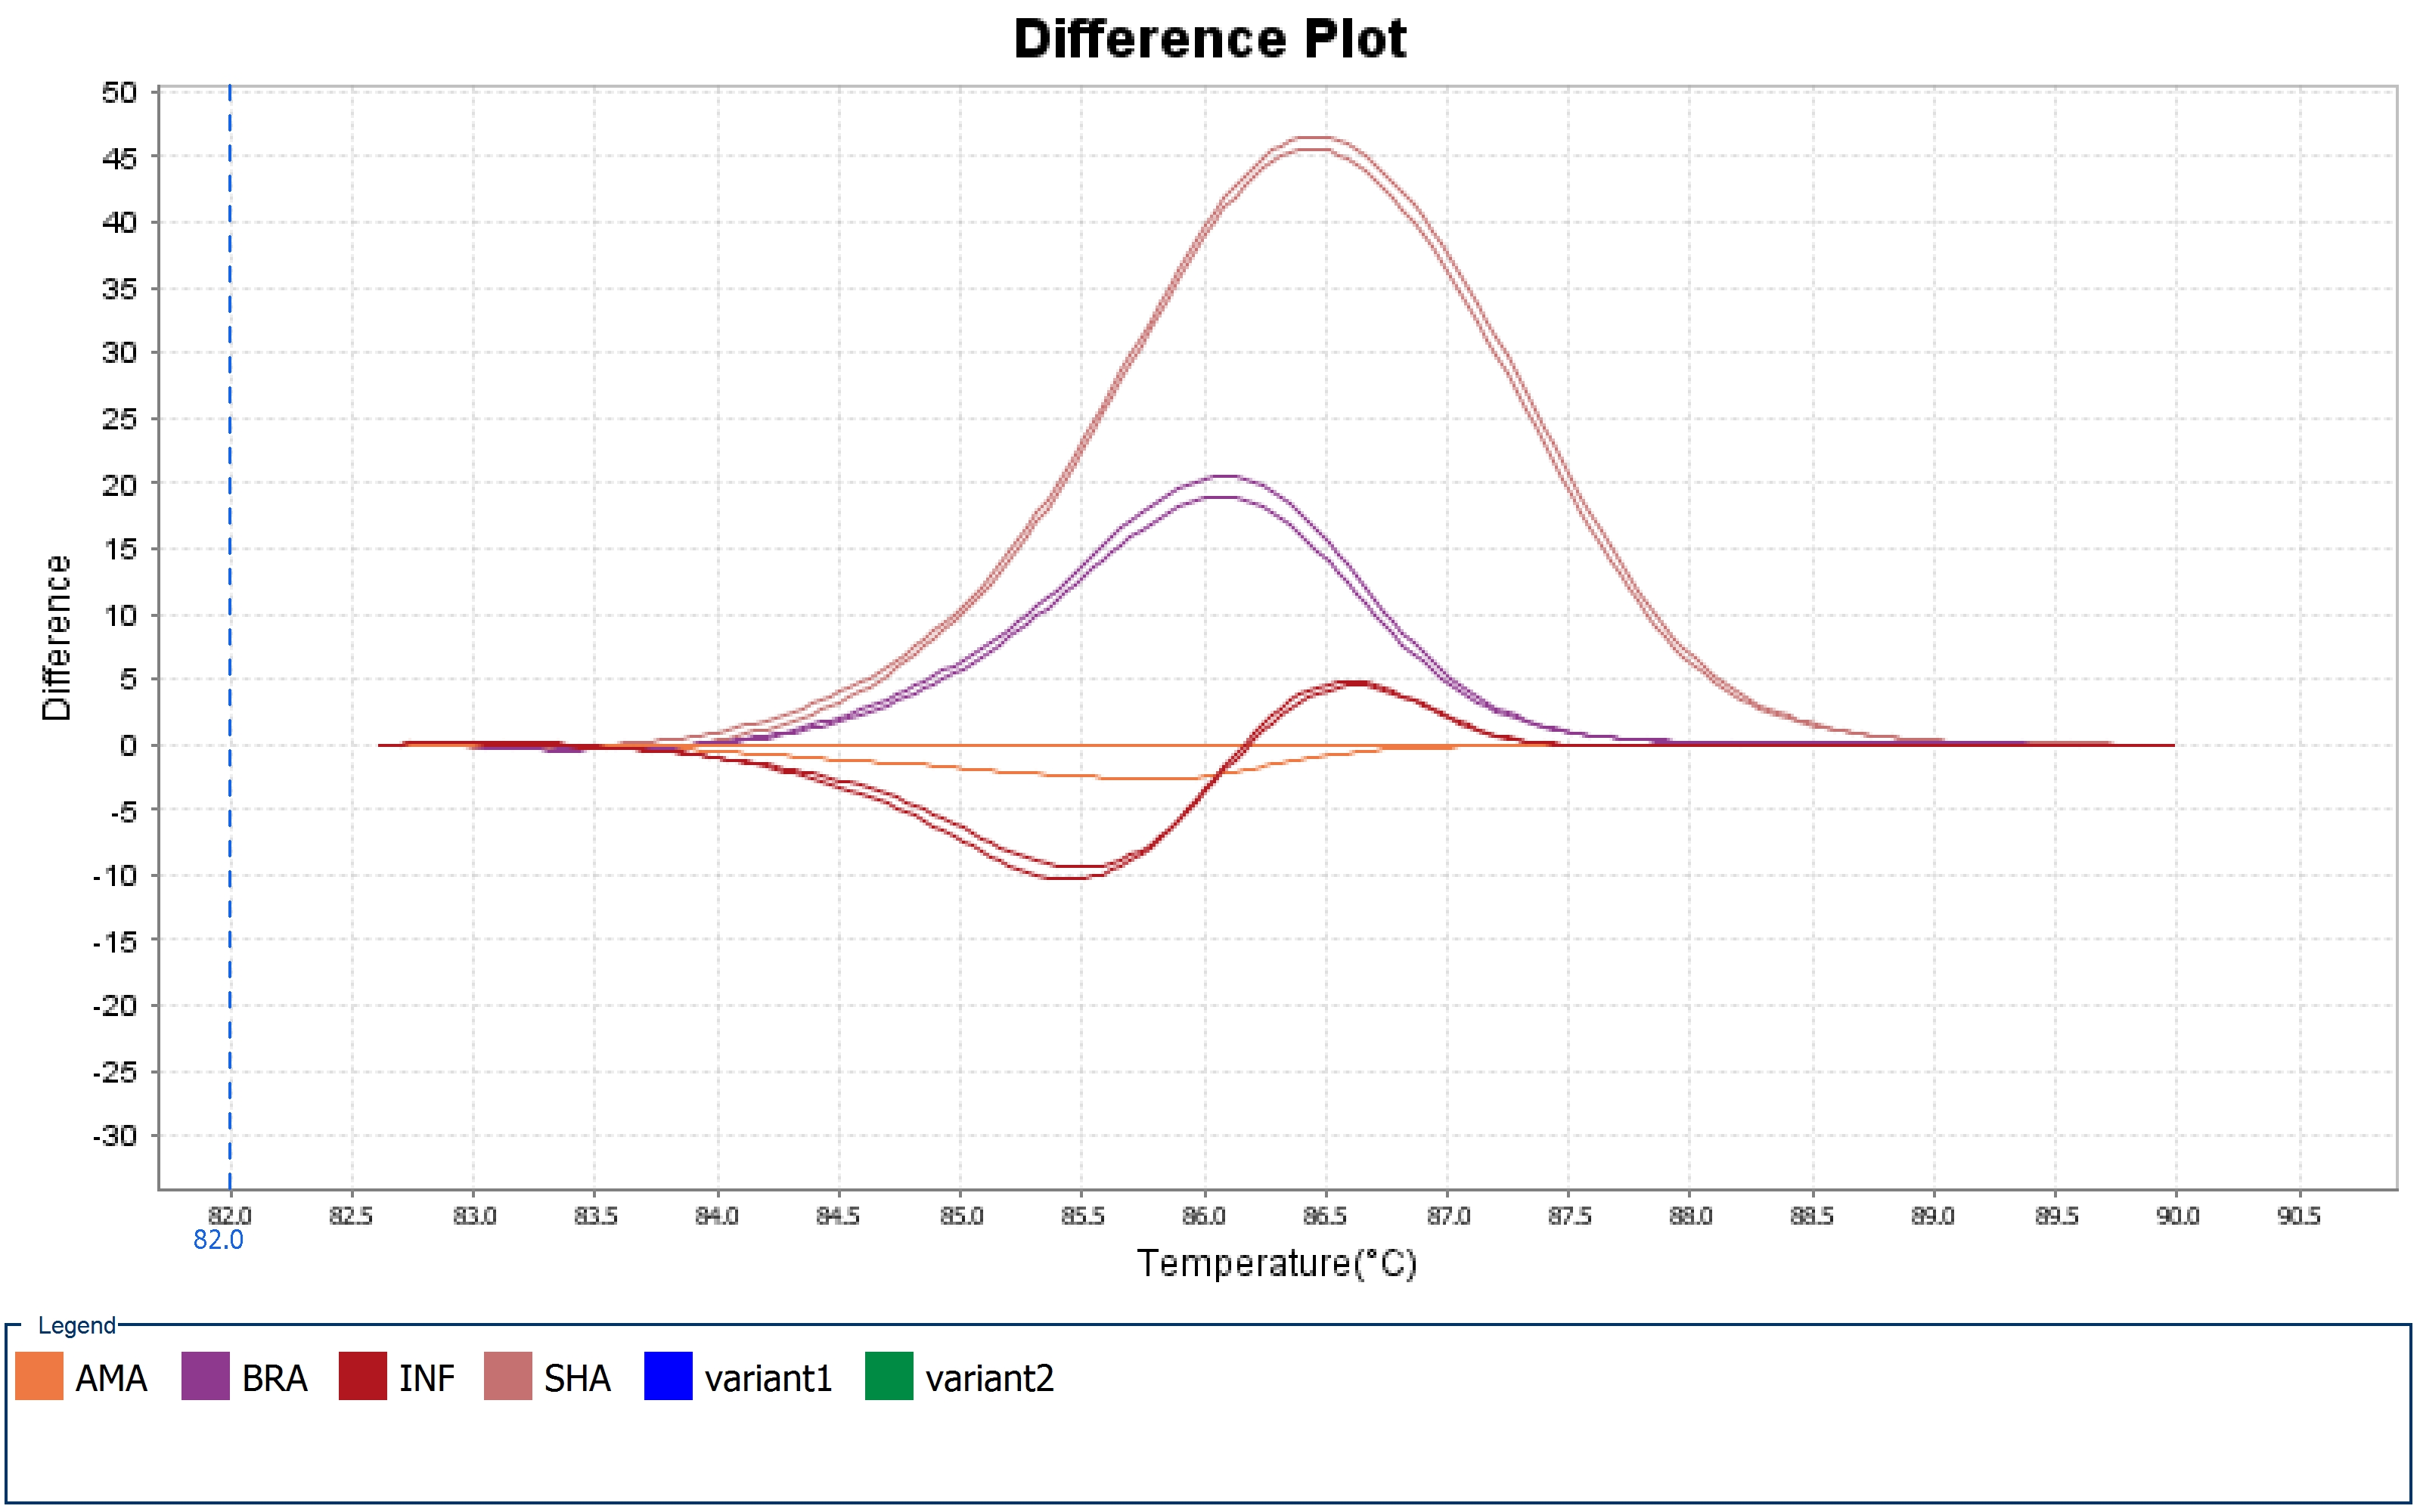
\includegraphics[width=.4\textwidth]{fig/Difference Plot.jpg}
        \caption{foto 1}
        \label{diffp}
        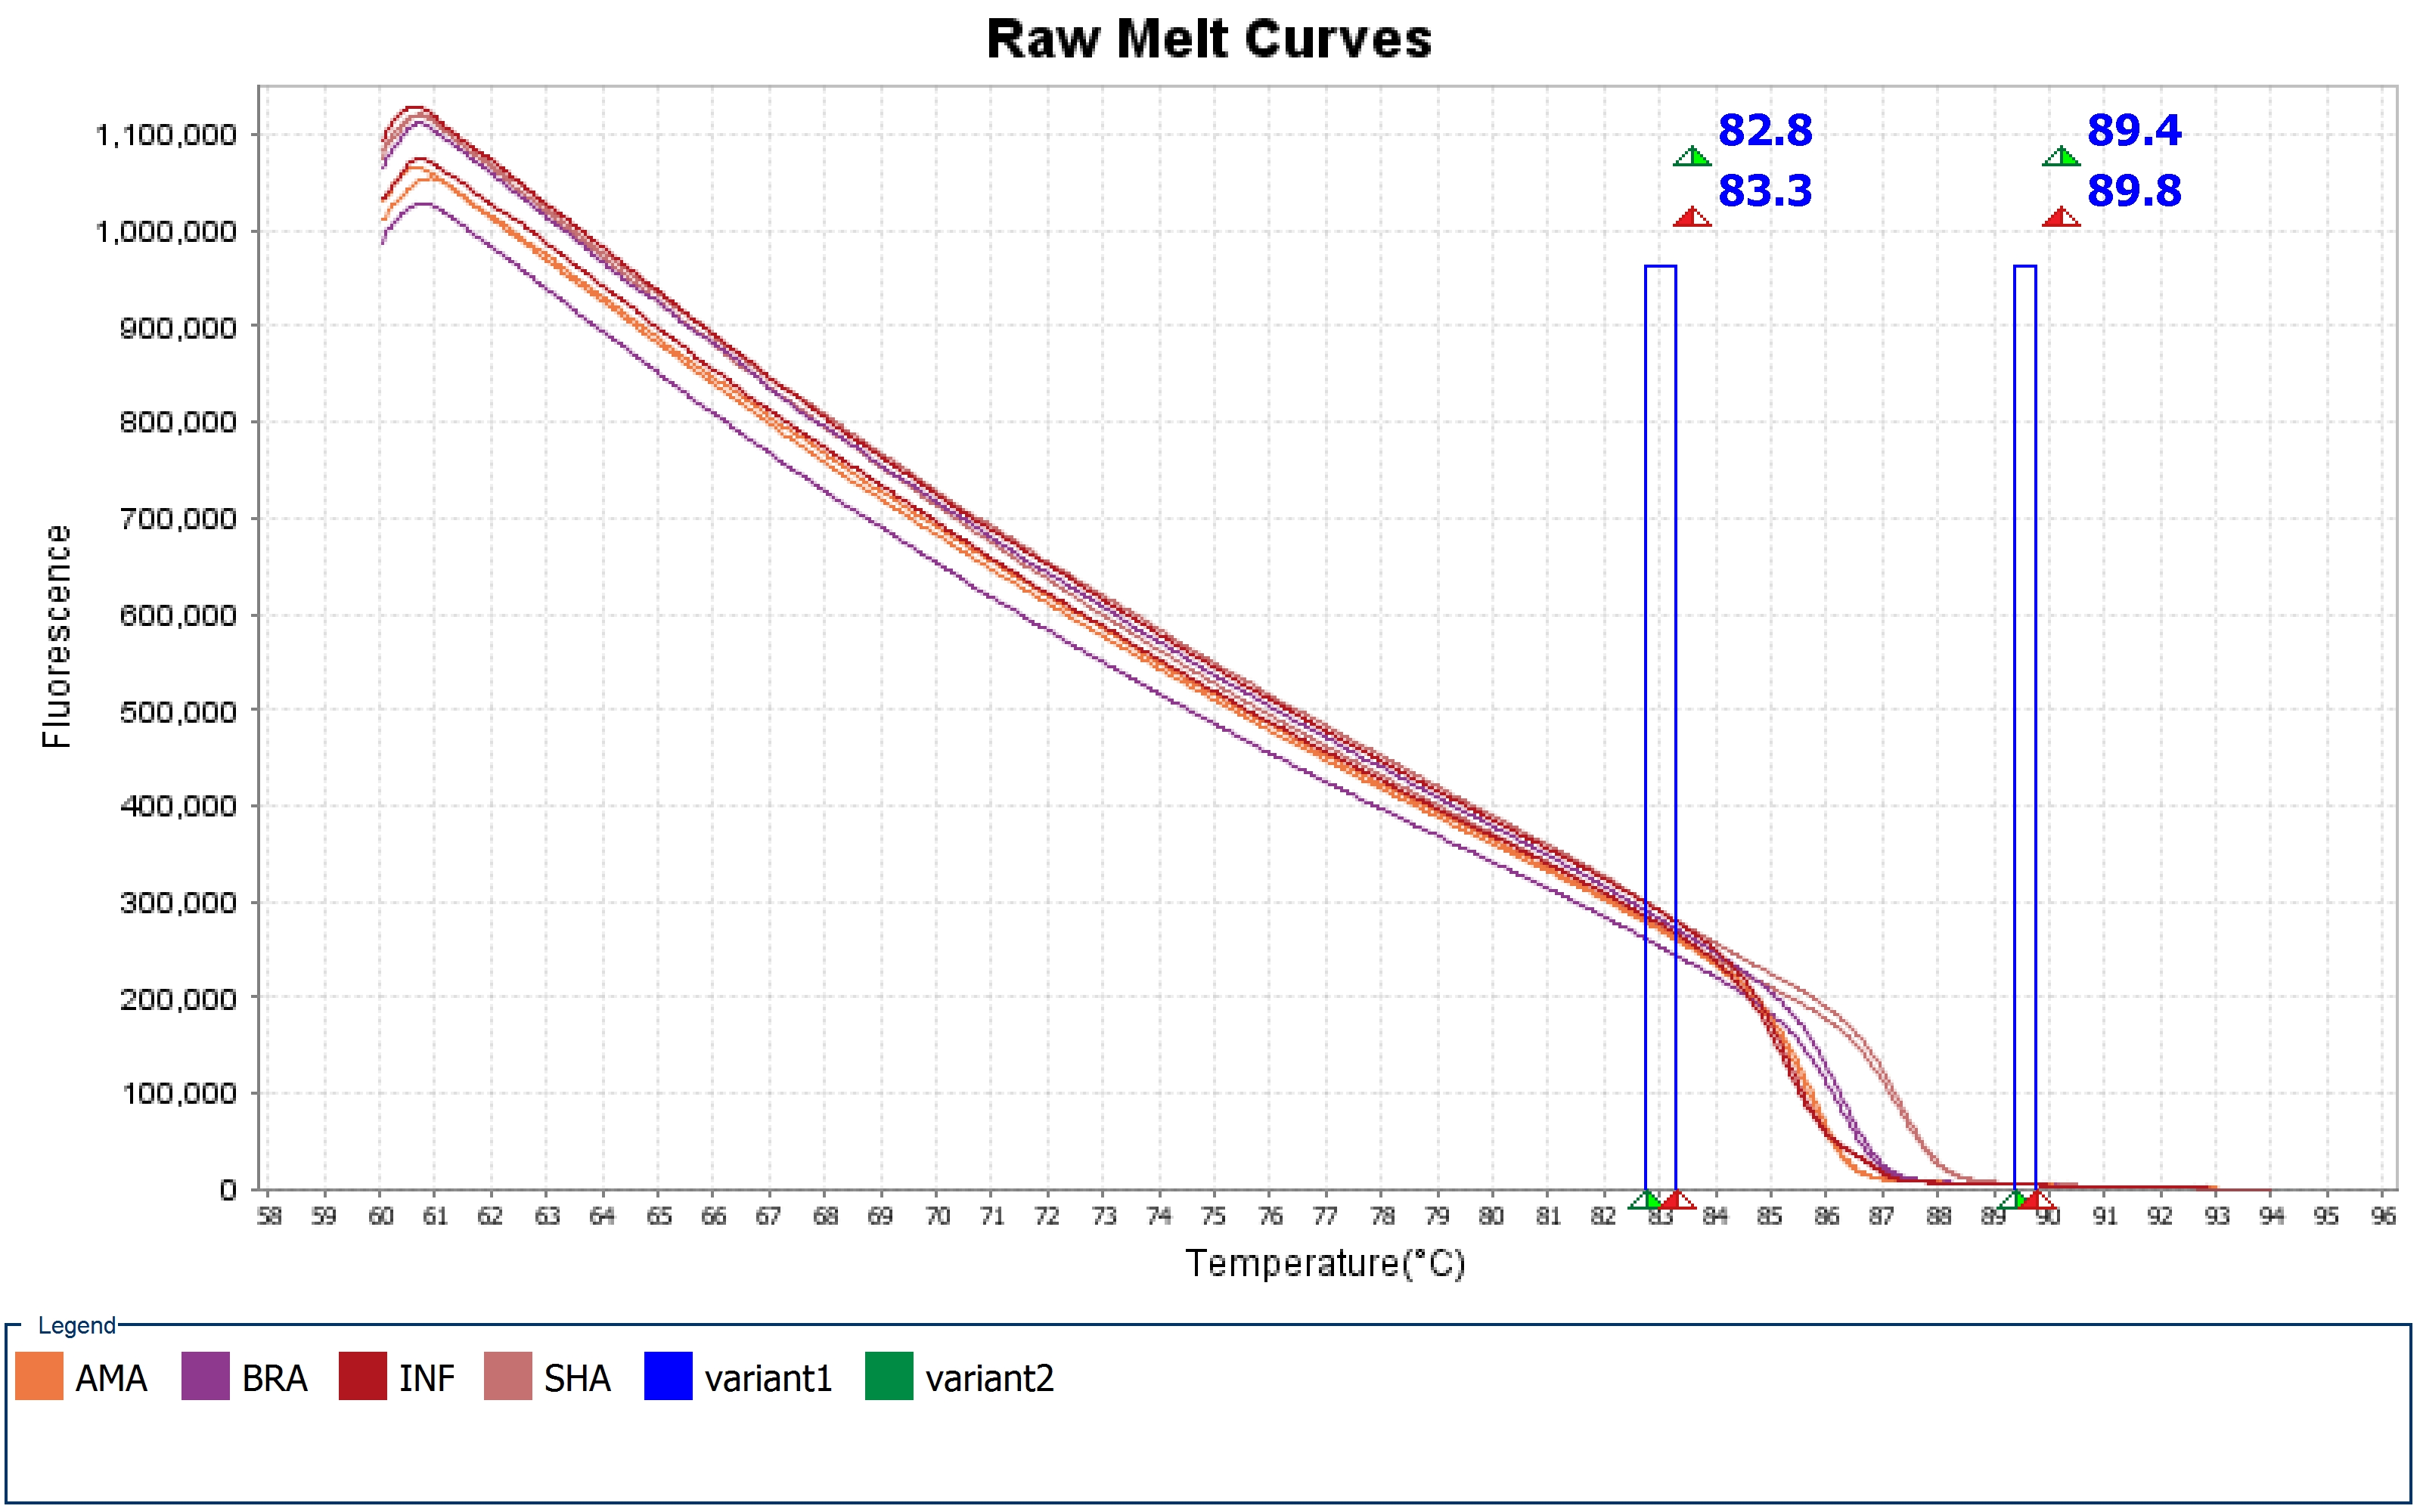
\includegraphics[width=.4\textwidth]{fig/Raw Melt Curves.jpg}
        \caption{Raw}
        \label{rawmelt}
\end{wrapfigure} %TODO: transformar imagens em uma prancheta, talvez não colocar
% como wrap fig... 

Primeiro, apenas com as amostras conhecidas, foram geradas as
\cref{dmeltc,diffp}. A
\cref{dmeltc} apresenta as curvas derivadas da fluorescência em função da
temperatura (derivative melt curves), nas quais os picos representam as
temperaturas de melting (Tm) específicas para cada amostra padronizada.

Para evidenciar as diferenças entre os perfis de melting das
amostras, foram geradas curvas de diferença (difference plots), apresentadas na
\cref{diffp}. 
É notável que cada espécie estudada
apresentou comportamento de melting único em comparação às demais. 

Por fim, a \cref{rawmelt} mostra as curvas normalizadas de reporter (normalised
reporter) em relação à
temperatura. Nesta é possível observar o padrão das amostras com \textit{L. (V.) shawi} e
\textit{L. (V.) brasilienses} que são visualmente distinguíveis. Já as curvas de
\textit{L. (L.) amazonensis} e \textit{L. (L.) infantum} são mais similares
entre si, embora facilmente distinguível das outras duas,  com
a maior diferença observável em valores pouco menores à \qty{87}{\celsius}.

\begin{wrapfigure}{L}{.45\textwidth}
        \centering
        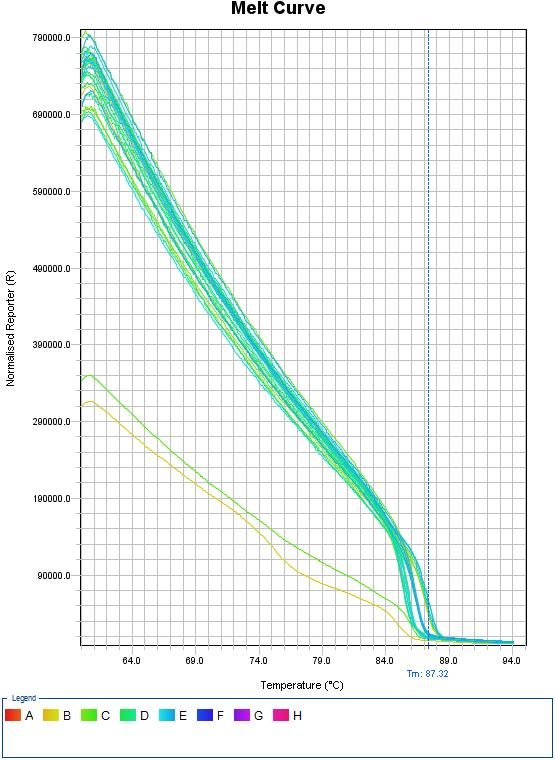
\includegraphics[width=.4\textwidth]{fig/Melt Curve.jpg}
        \caption{foto 1}
        \label{meltc}
        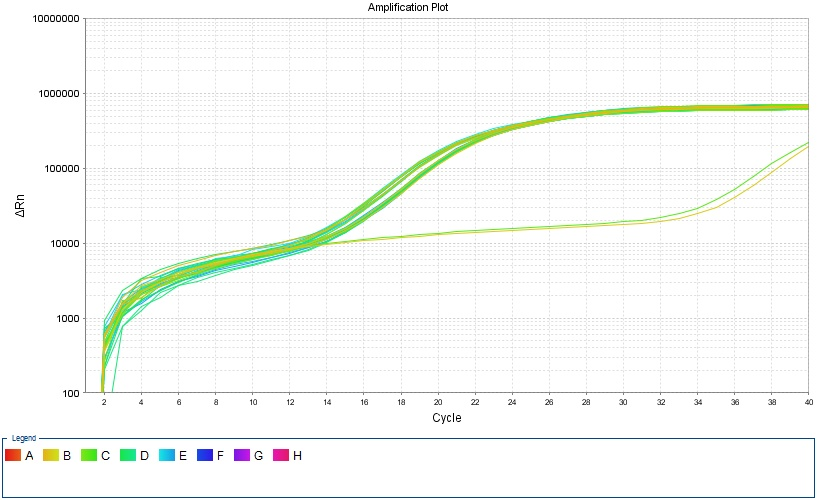
\includegraphics[width=.4\textwidth]{fig/Amplification Plot.jpg}
        \caption{foto 1}
        \label{amplip}
\end{wrapfigure}

As \cref{meltc,amplip} correspondem aos resultados da segunda reação de PCR em
tempo real, realizada com um conjunto de amostras desconhecidas acompanhadas de
controles positivos e negativos. A curva de melting apresentada na \cref{meltc}
revela que a maioria das amostras desconhecidas apresenta perfis de dissociação
compatíveis com os observados nas amostras padronizadas discutidas anteriormente
(\cref{dmeltc,diffp}), especialmente em relação aos valores de Tm, que podem ser
claramente identificados para cada amostra no gráfico.

Como esperado, duas curvas presentes na \cref{meltc} exibem perfis atípicos do
padrão observado nas curvas com as amostras conhecidas, estas duas curvas são
referentes aos dois poços com controle negativo. Isto é corroborado ao avaliar
as mesmas curvas na \cref{amplip}, que mostra as curvas de amplificação
correspondentes à mesma placa, em que esses dois poços não apresentaram aumento
significativo na fluorescência, comportamento compatível com o esperado para os
controles negativos incluídos na reação.

Ademais, na região de \qty{85}{\celsius}-\qty{88}{\celsius} da \cref{meltc} é
possível observar três padrões evidentemente diferentes e mais um que se
diferencia à pouco menos que \qty{87}{\celsius}. Estes são os mesmos quatro
padrões observados nas amostras conhecidas (\cref{rawmelt}).
>>>>>>> 3568cdef6f851064c18dd7f0daa39c3c1214baf9
